\section{Simulations}

In this section, the applied simulation framework and the implemented simulations are presented for the quadrotor flip maneuver, followed by the achieved results. The simulations are based on the dynamic model of a Bitcraze Crazyflie 2.1 miniature quadcopter which we use for demonstrating the experimental results in Section \ref{sec:exp}, as well. The nonlinear equations of motion are defined in Section \ref{sec:model}, and the physical parameters of the drone are shown in Table \ref{tab:params}, obtained from \cite{Forster}.

\begin{table}[!b]
    \centering
    \setlength{\tabcolsep}{1.5pt}
    \caption{Physical parameters of the Crazyflie 2.1 quadcopter.}
    \label{tab:params}
    \begin{tabular}{|l|c|rl|}
        \hline
        \phantom{o}Mass &\phantom{o} $m$ \phantom{o}& 0.028&g \\
        \hline
        \phantom{o}Propeller-to-propeller length \phantom{o}&\phantom{o} $l$\phantom{o} & 92&mm\\
        \hline
        \multirow{3}{*}{\phantom{o}Diagonal inertia elements} & \phantom{o}$J_{xx}$\phantom{o} & $1.4\cdot 10^{-5}$&kgm$^2$\\
         \cline{2-4}
        &\phantom{o} $J_{yy}$ \phantom{o}& $1.4\cdot 10^{-5}$&kgm$^2$\\
        \cline{2-4}
        & \phantom{o}$J_{zz}$\phantom{o} & \phantom{o}$2.17\cdot 10^{-5}$&kgm$^2$\phantom{o}\\
        \hline
        \phantom{o}Thrust coefficient & $k$ & $2.88\cdot 10^{-8}$ & Ns$^2$\\
        \hline
        \phantom{o}Drag coefficient & $b$ & \phantom{o}$7.24\cdot 10^{-10}$ & Nms$^2$\phantom{o}\\
        \hline
    \end{tabular}
\end{table}

After some literature survey about drone simulators such as \cite{airsim2017} and \cite{flightmare2020}, we decided to choose an OpenAI Gym environment based on PyBullet \cite{gym}. This framework is written in Python language, contains the physical model and parameters of the Bitcraze Crazyflie 2.1, has built-in multi-agent control, and tuned PID controller for the drone. There are also some simple examples for trajectory tracking, and reinforcement learning with a swarm of drones.

All of the simulation code used in this work is available at GitHub\footnote{\url{https://github.com/antalpeter1999/TDK2021}}, the Python code is in the simulations/crazyflie-demo-simulation repository, and the Matlab code is in the trajectory-design repository.

\subsection{Optimized open-loop control}\label{sec:opensimu}
Based on the control approach presented in Section~\ref{sec:flip}, we implemented the open-loop flip controller which evaluates the five sections of the parametrized motion primitive. For the optimization of the parameters defined in \eqref{eq:openparams}, we utilize the Bayesian Optimization Python module \cite{bayesopt}.% The source code is available at \url{https://github.com/antalpeter1999/gym-pybullet-drones-0.5.2}.

The simulation starts with hovering for about 0.1 s, followed by executing the open-loop maneuver, and then switching back to PID control to stabilize the drone and bring back to the initial setpoint. The objective function of the optimizer uses the same simulation, and returns the norm of the final state error, as it is characterized in \eqref{eq:optim}. The optimal parameters were calculated with Bayesian optimization, using 250 random initial function evaluations and 1000 iterations. The numerical values of these are
\begin{align}\label{eq:optparam}
P^*=\begin{bmatrix}
U_1^* & t_1^* & t_3^* & U_5^*& t_5^*
\end{bmatrix} ^\top =  \begin{bmatrix}
17.5 & 0.12 & 0.16 & 17.95 & 0.075
\end{bmatrix}^\top,
\end{align}
where the unit of the collective accelerations $U_i^*$ is m/s$^2$, and the time is in seconds. It is simple to convert the collective acceleration to collective thrust, 
\begin{equation}
    F = m U,
\end{equation}
where $m$ is the mass of the quadcopter. Simulation results are displayed in Figure \ref{fig:opensimu}, using the optimal parameter vector and a set of near-optimal parameters, as well. On the left plot, the position of the quadcopter during the flip is shown, with snapshots from the simulation. The end of the optimal maneuver is around the coordinate $(x, z)=(-0.4, 0)$~m with near-zero pitch angle, thus the final state error is only significant in the $x$ position. From that point, a PID controller stabilizes the drone and controls to the origin. On the right, the trajectory of the pitch angle in Euler representation, the angular velocity, and the collective thrust as a control input are shown, where the five sections defined in Section~\ref{sec:flip} can be recognised clearly. The figure illustrates that even small deviations from the optimal parameter set (<10\%) result in significantly decreasing performance.

\begin{figure}[!h]
\centering
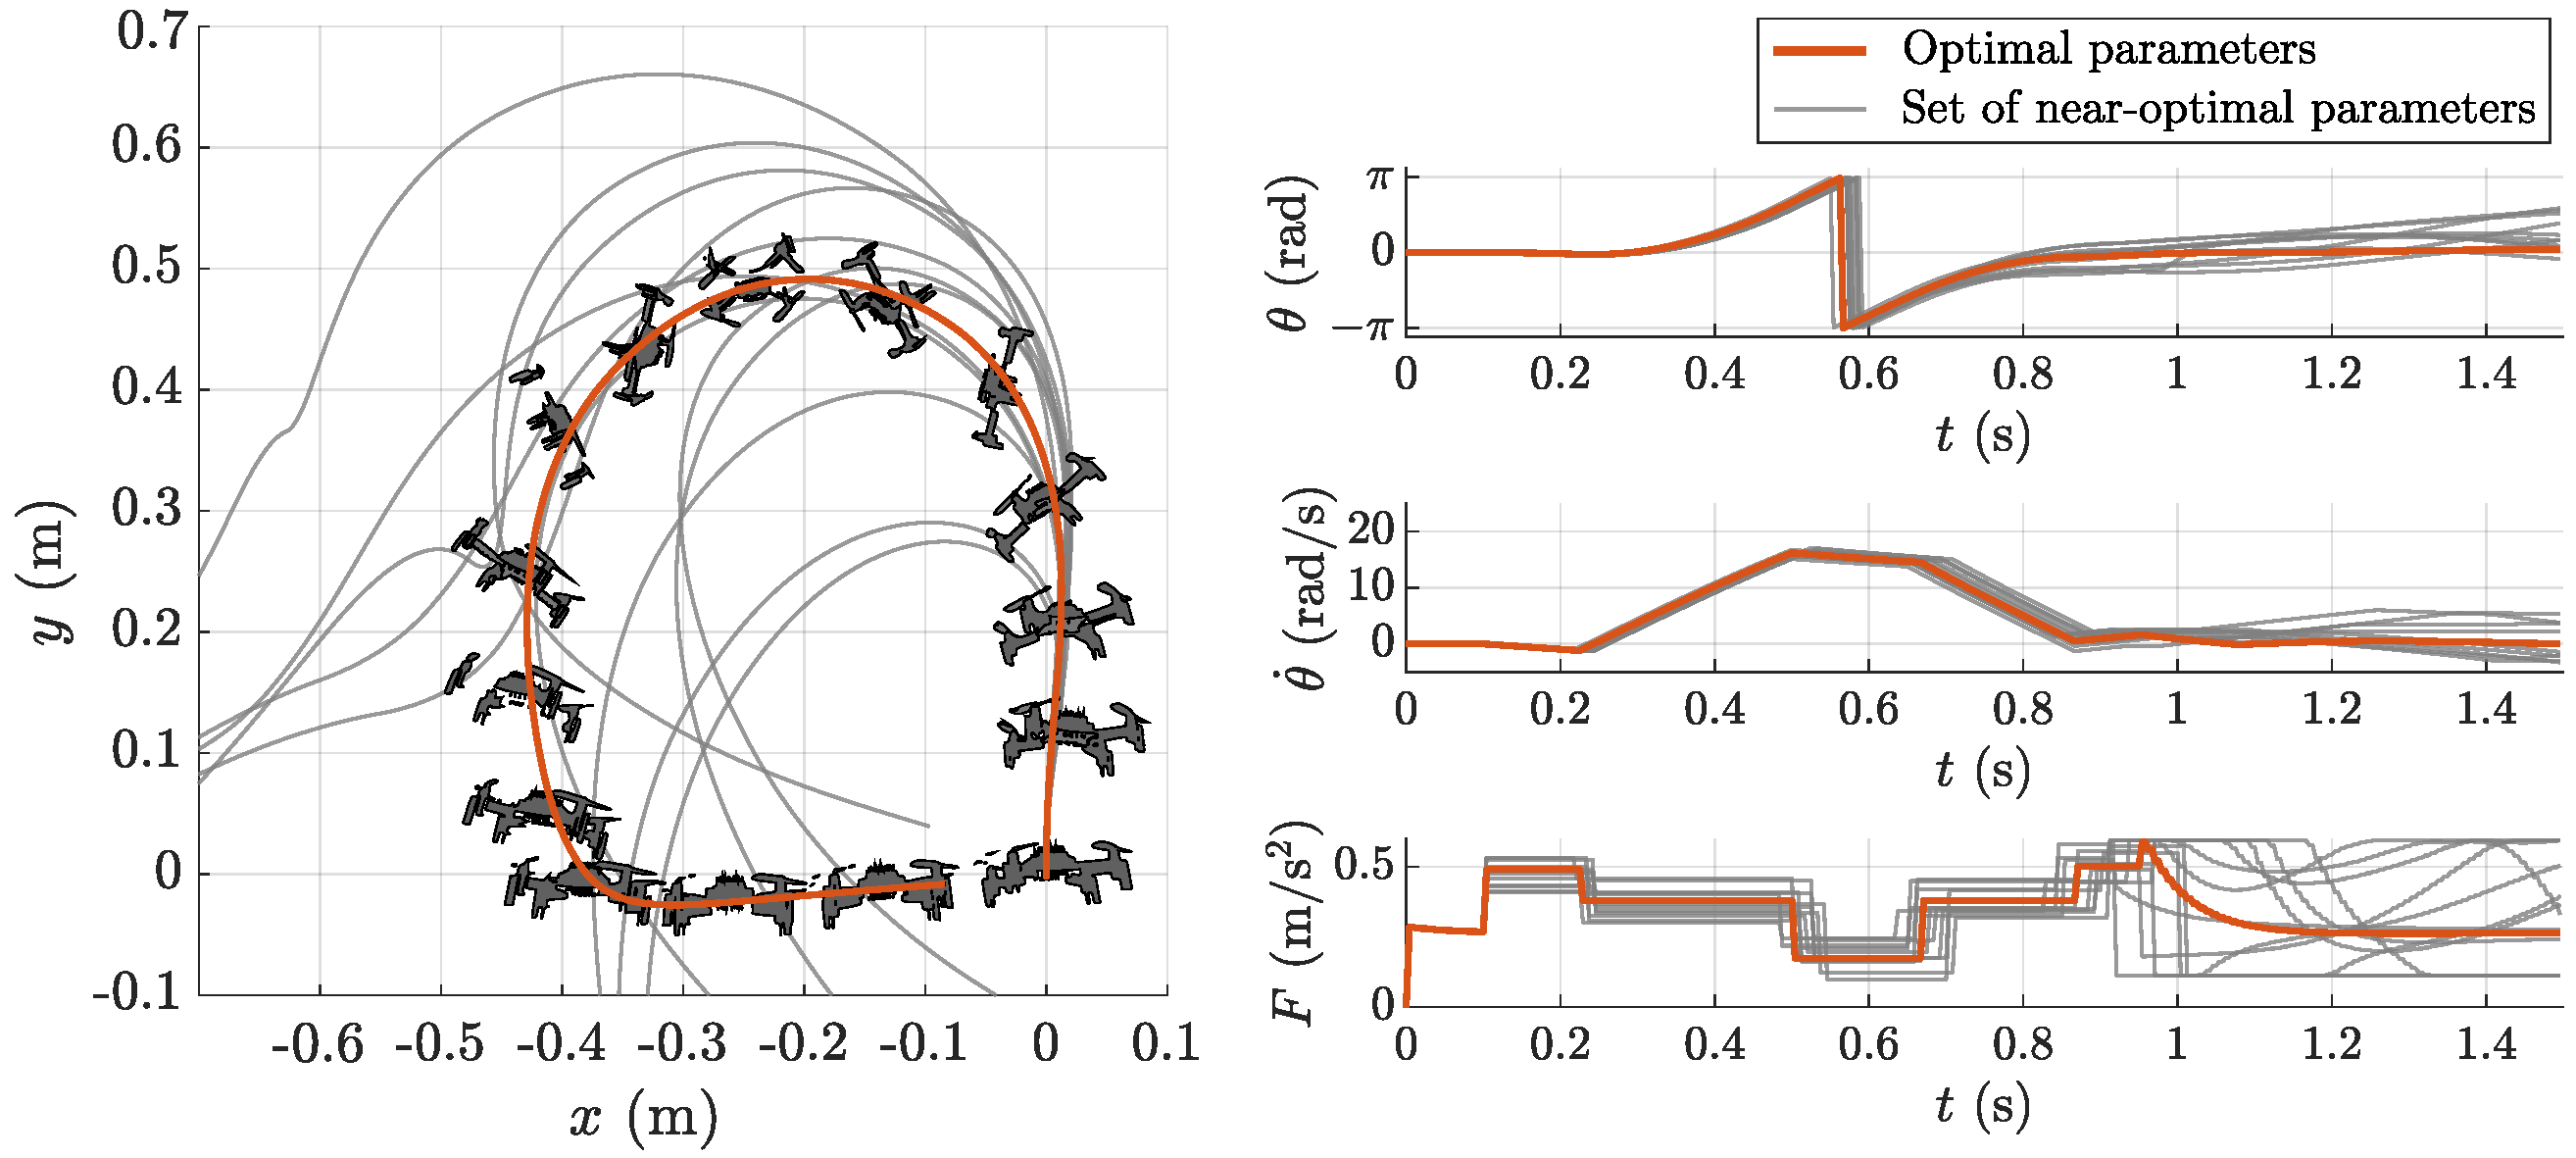
\includegraphics[width=\linewidth]{Fig/opensimu2.pdf}
\caption{Open-loop backflip simulation results: the position is displayed on the left, and the pitch angle $\theta$, pitch angular velocity $\dot{\theta}$, and collective thrust $F$ on the right. Orange lines represent the simulation with optimal parameters in \eqref{eq:optparam}, and grey lines represent the result of small changes in the parameter set.}\label{fig:opensimu}
\end{figure}



%\begin{figure}
%\centering
%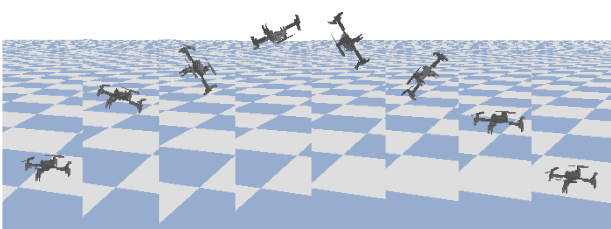
\includegraphics[width=.2\linewidth]{Fig/pics.png}
%\caption{Frames from the flip maneuver simulation video.}\label{fig:flipsimu}
%\end{figure}

\pagebreak
\subsection{Trajectory planning and geometric control}

The second control approach to perform a flip maneuver is trajectory planning and reference tracking with geometric control. Based on the results of the flip with open-loop control, the parameters of the reference pitch trajectory are chosen to $\alpha=20$~1/s, $\beta=0.45$~s, as illustrated in Figure \ref{fig:attref}. In the quadratic programming problem \eqref{eq:quadprog} we use the following parameters:
\begin{align}
    \mathcal{X}:\;\begin{bmatrix} x_- \\ x_+ \\ z_- \\ z_+ \end{bmatrix} =  \begin{bmatrix} -0.6 \\ 0 \\ -0.05 \\ 0.45 \end{bmatrix}\;\mathrm{m};\quad \mathcal{U}:\;F \in [0,0.64]\;\mathrm{N}; \quad T_s = 1/480\;\mathrm{s}.
\end{align}
The maximal collective thrust $F_\mathrm{max}=0.64$ N is from \cite{Forster}, and the position bounds are chosen such that the trajectory is feasible, and the quadcopter does not get too far from the initial point. The duration of the flip is chosen to $T=0.9$~s, thus the number of simulation steps is $N=T/T_s=432$. The quadratic optimization problem is solved by the \verb+quadprog+ function of Matlab with negligible computation time. The result is the optimal control input and reference position sequence given in the discrete time instants.

The official Crazyflie 2.1 firmware has built-in trajectory evaluation algorithm for 7th degree polynomials\footnote{\url{https://www.bitcraze.io/documentation/repository/crazyflie-firmware/master/functional-areas/trajectory_formats/}}, therefore we fit such functions to the optimal position sequence, and use it as the reference for the flip maneuver. As both the $x$ and $z$ solution are smooth, the 7th degree polynomials can be fitted with almost zero error using the Curve Fitting Toolbox of Matlab.

The quadcopter follows the designed reference trajectory with geometric tracking control, based on the control law \eqref{eq:geomlaw} and error terms \eqref{eq:geomerrors}. The diagonal gain matrices were determined based on grid search and considering that the Mellinger controller \cite{mellinger2011} with a similar control law is part of the official Crazyflie 2.1 firmware\footnote{\url{https://www.bitcraze.io/documentation/repository/crazyflie-firmware/master/functional-areas/sensor-to-control/controllers/}}. The numerical values are
\begin{align*}
    K_r = \mathrm{diag}\left(\begin{bmatrix}
    0.5 \\ 0.5 \\ 1.25
    \end{bmatrix} \right);\quad K_v = \mathrm{diag}\left(\begin{bmatrix}
    0.2 \\ 0.2 \\ 0.8
    \end{bmatrix} \right);\quad K_R = 0.08 I_{33}; \quad K_\omega = 0.002 I_{33},
\end{align*}
 where the result of diag$(\cdot)$ is a $3\times 3$ matrix with the argument vector in the diagonal, and $I_{33}$ is the $3\times 3$ identity matrix.
 
 The simulation results of the trajectory planning and reference tracking with geometric control are displayed in Figure \ref{fig:geomsimu}. Similarly to the open-loop approach, the maneuver starts and ends at hovering, but in this case the stabilizing controller is also the geometric control with position and yaw setpoint. At the beginning of the maneuver, the controller is switched from yaw to pitch reference to follow the specified reference trajectory. The left plot illustrates the reference and simulated pose of the quadcopter during the backflip maneuver, and the right plot contains the trajectory of the pitch angle, angular velocity and collective thrust control input. The trajectory of both the angular velocity and the thrust input are smooth, opposed to the discontinuous angular acceleration and thrust of the open-loop control. In the discontinuities of the control input the unmodeled transient behaviour of the actuator dynamics can be significant, therefore the geometric control approach is more robust to such uncertainties compared to the open-loop method. 
 
\begin{figure}
    \centering
    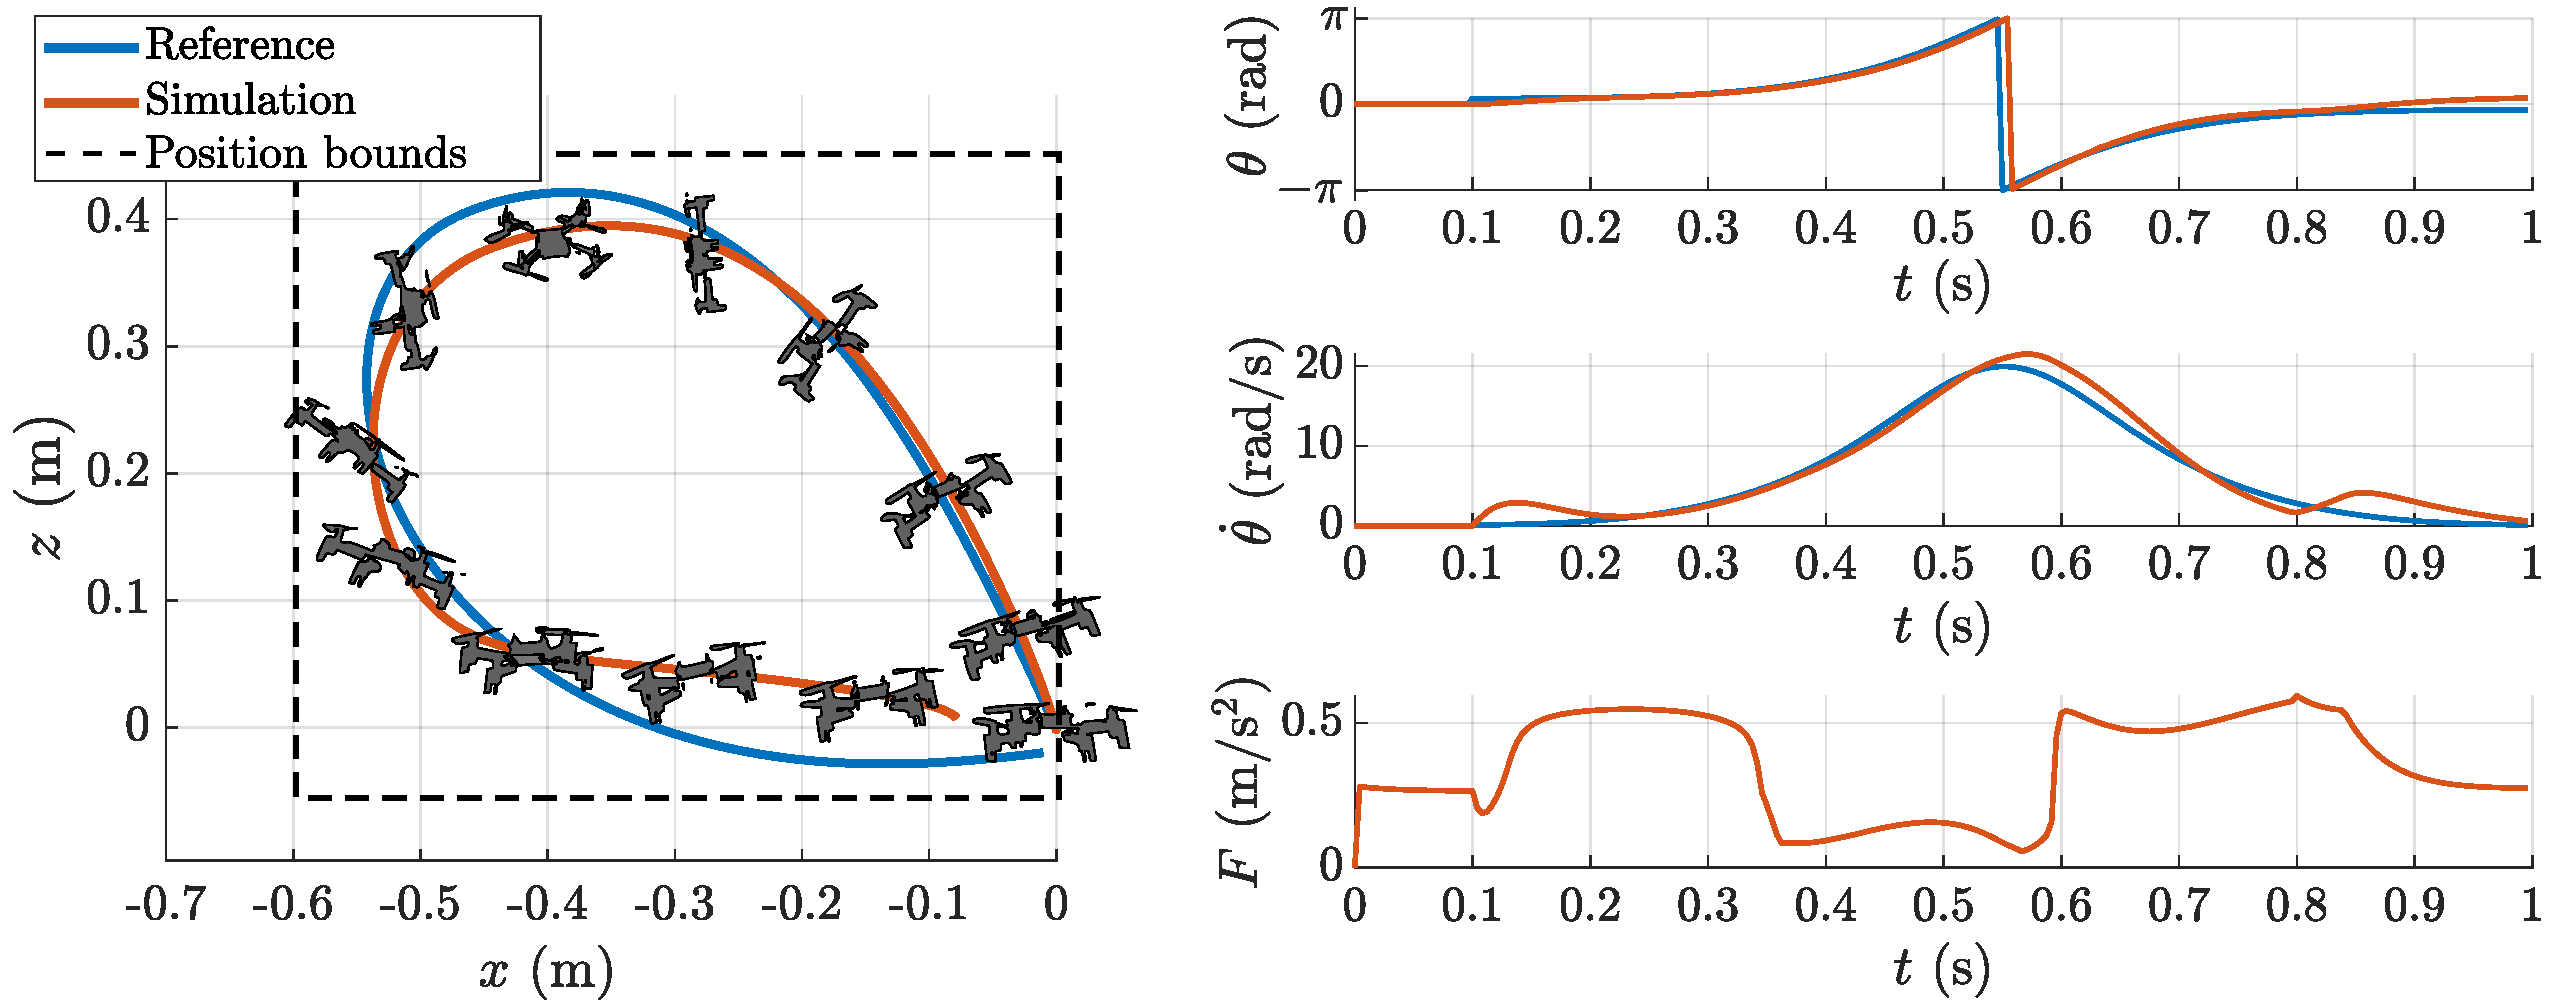
\includegraphics[width=\linewidth]{Fig/geomsimu.pdf}
    \caption{Backflipping simulation results with geometric control: position and attitude on the left, the pitch angle $\theta$, pitch angular velocity $\dot{\theta}$, and collective thrust $F$ on the right.}\label{fig:geomsimu}
    \end{figure}

\begin{figure}
    \centering
    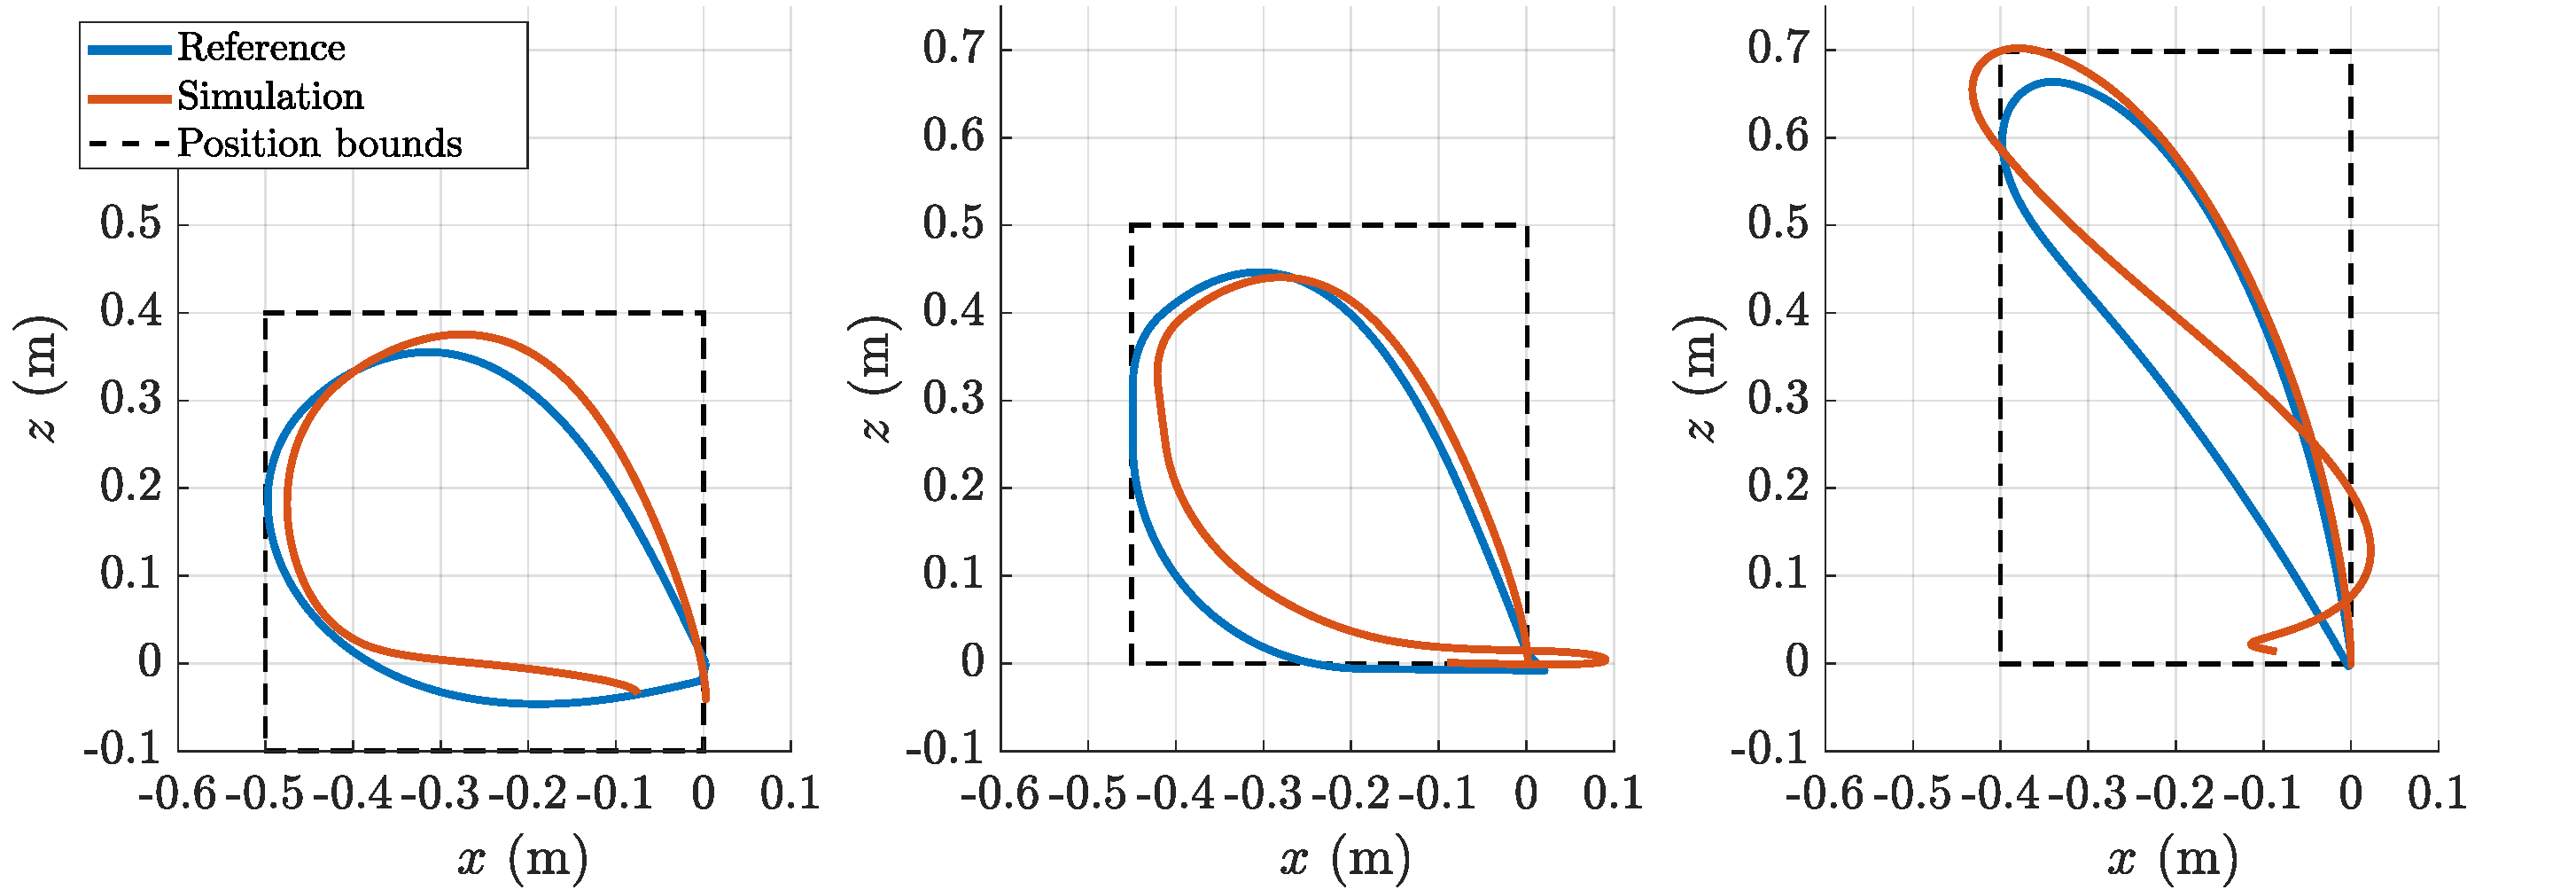
\includegraphics[width=\linewidth]{Fig/geomsimu2.pdf}
    \caption{Backflipping simulation results with geometric control. The position reference constraint is different for each simulation, illustrated by the dashed lines.}\label{fig:geomsimu2}
\end{figure}
 
 It can be seen that the orientation reference tracking is more precise than the position. Fast and accurate attitude tracking is required to stabilize the quadcopter, however, the reference trajectory is designed with the assumption that the attitude equals to the reference at all times, therefore there are more significant errors in the position.
 
 
